\chapter{Анализ систем составления расписания в ВУЗах} \label{ch1}

Проблема составления расписания не нова, и существует множество средств, призванных упростить её решение. В интернете можно найти онлайн-календари с возможностью совместного редактирования, системы управления бизнес-процессами и программы генерации расписания для разного рода предприятий. Но далеко не все из них могут быть использованы в качестве полноценной системы составления расписания сессии для университета, поэтому в параграфе \ref{ch1:sec1} рассматриваются требования к системе составления расписания сессии СПбПУ.

На рынке существует отдельная ниша систем составления расписания для ВУЗов, и в параграфе \ref{ch1:sec2} рассматриваются её русскоязычные представители, а в параграфе \ref{ch1:sec3} - зарубежные. Далее приведено сравнение таких систем и анализ их преимуществ и недостатков для решения конкретной задачи - составления предварительного расписания сессии в университете.

\section{Требования к системе составления расписания сессии} \label{ch1:sec1}

\subsection{Учёт семестрового расписания СПбПУ}

Важным аспектом системы составления расписания сессии СПбПУ является учёт занятости аудиторий и преподавателей. Бывают ситуации, когда сессия для некоторых учебных групп начинается в тот момент, когда у других групп всё ещё проводятся семестровые занятия. Чтобы иметь возможность составлять расписание сессии, которое не ставит проведение аттестаций в занятые по семестровому расписанию аудитории, необходимо обращаться c помощью API к официальному расписанию занятий ~\cite{ruz}. 

\subsection{Роли пользователей системы}
Одним из требований к системе сбора сведений является выделение двух ролей пользователей:
\begin{itemize}
	\item Администратор - пользователь, который сообщает системе сведения о сессии, аудиториях и о плане экзаменов, а также инициирует процесс генерации расписания.
	\item Преподаватель - пользователь, который сообщает системе о собственных пожеланиях к проведению своих экзаменов.
\end{itemize}

Рассмотрим возможности этих типов пользователей подробнее. На диаграмме на рисунке \ref{fig:usecse1} показаны возможности преподавателя.
Преподаватель может участвовать в составлении расписания, указав даты, дни недели и время, когда он доступен или не доступен для проведения аттестаций, необходимые типы аудиторий, своих ассистентов и пожелания по компоновки групп по дням.

\begin{minipage}{\textwidth}
	\centering
	\vspace{\mfloatsep} % интервал  	
	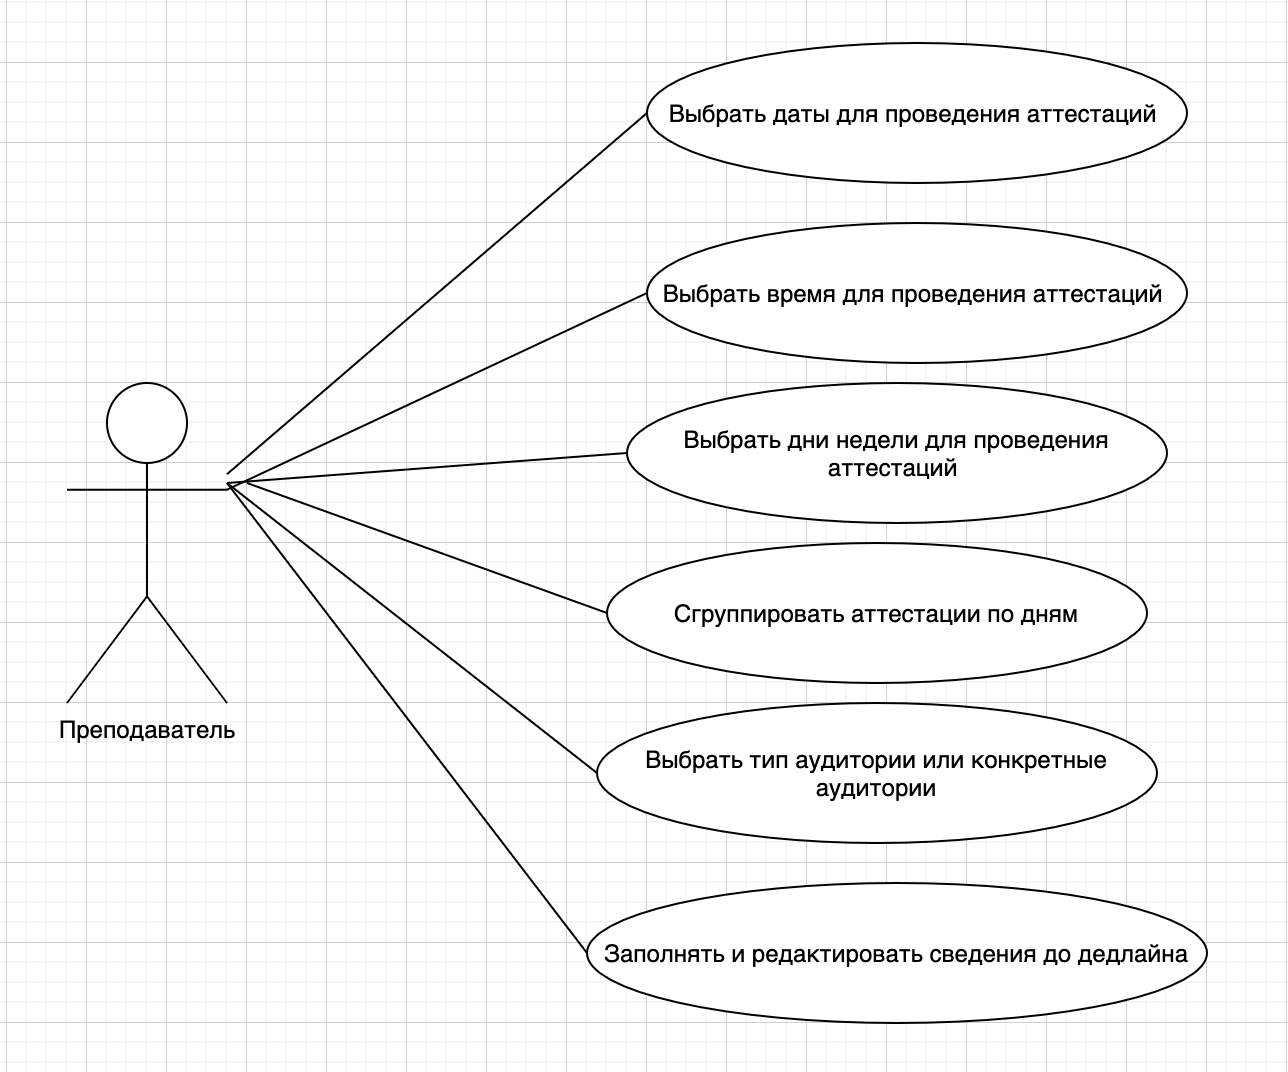
\includegraphics[scale=0.6, keepaspectratio=true] {my_folder/images/usecase1}
	\captionof{figure}{Use case диаграмма ППС}\label{fig:usecse1}  
	\vspace{\mfloatsep} % интервал  	
\end{minipage}

Возможности администратора показаны на диаграмме на рисунке \ref{fig:usecse2}.
Администратор заполняет общие сведения о сессии, такие как даты, время, доступные аудитории с указанием, сколько в них мест и есть ли там проектор и компьютеры и предстоящие экзамены по группам и преподавателям. Также, могут быть указаны аттестации, для которых уже определено время и место проведение. Это актуально, например, для событий, проводимых другими подразделениями университета. В возможности администратора помимо вышесказанного входит генерация формы сбора предпочтений преподавателей. 

\begin{minipage}{\textwidth}
	\centering
	\vspace{\mfloatsep} % интервал  	
	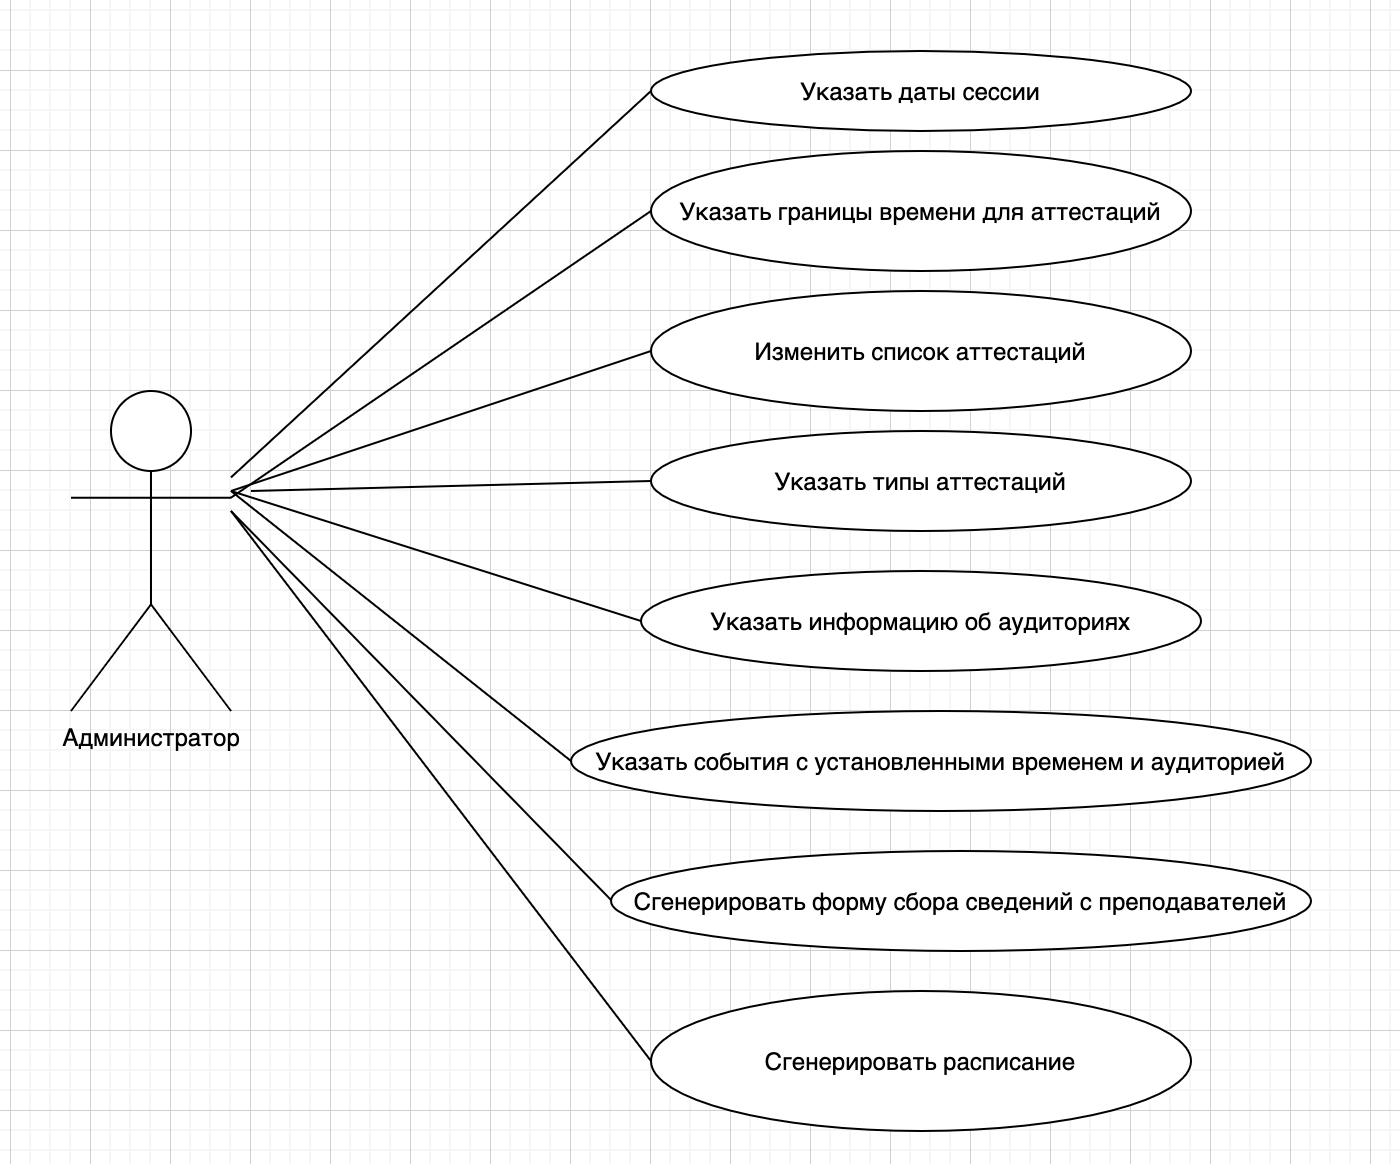
\includegraphics[keepaspectratio=true,scale=0.6] {my_folder/images//usecase2}
	\captionof{figure}{Use case диаграмма администратора}\label{fig:usecse2}  
	\vspace{\mfloatsep} % интервал  	
\end{minipage}

Таким образом, когда администратор заполнит все вышеперечисленные поля формы, в системе уже будет минимальный набор данных, необходимый для составления расписания. 
Далее, преподаватели могут заполнять свои формы с пожеланиями к своему расписанию. Незаполненная преподавателем форма не будет являться проблемой для системы. Пустая форма по умолчанию приравнивается к готовности преподавателя проводить экзамены и зачёты в любой день, в любое время и в любой аудитории. 

\section{Обзор российских систем составления расписания} \label{ch1:sec2}

\subsection{1С: ХроноГраф Расписание} 
Фирма <<1С>>, занимающаяся разработкой ПО для бизнеса и образования, в качестве системы для автоматизации учебного планирования и составления расписания в разного рода организациях предлагает свою программу <<1С: ХроноГраф Расписание>>~\cite{1с}.
<<1С: ХроноГраф Расписание>> позволяет:
\begin{itemize}
	\item cоставлять понедельное расписание организации или отдельных её подразделений;
	\item задавать периоды обучения с учётом нерабочих дней, каникул и разбиением на четные и нечётные недели;
	\item создавать черновое расписание, используя функцию <<Предварительный расчёт>>.
\end{itemize}

Основной проблемой данной программы является несовместимость с другими платформами. <<1С: ХроноГраф Расписание>> - однопользовательская программа, и нельзя интегрировать её с web-приложением для возможности сбора данных напрямую от пользователей. Сложность составления расписания сессии в этой системе обуславливается также её ориентированностью на составление расписания по неделям без учёта специфики проведения аттестаций.

\subsection{Avtor}% сокращения не вводят в заголовках! 
Программа Avtor (<<АВТОРасписание>>) ~\cite{avtor} имеет несколько версий для различных учебных заведений: общеобразовательных школ, колледжей, техникумов, профессиональных училищ и ВУЗов. Это позволяет в подстроиться под специфику расписания конкретного типа образовательного учреждения, что является одним из её конкурентых преимуществ.

<<АВТОРасписание>> имеет достаточно широкий спектр применений. Этот программный продукт позволяет
\begin{itemize}
	\item cоставлять понедельное расписание для учебных групп с минимальным количеством окон;
	\item cоставлять расписание преподавателей с минимальным количеством окон;
	\item оптимально размещать занятия по аудиториям, учитывая их вместимость и оснащённость необходимым оборудованием;
	\item учитывать пожелания сотрудников к своему расписанию;
	\item разделять учебные группы на подгруппы;
	\item вносить ручные корректировки в расписание.
\end{itemize}

Преимуществом этой программы помимо прочего является возможность публиковать расписание обучающихся и преподавателей из самой системы <<Автор>> на сайте, внутреннем портале или на мультимедийных стендах образовательной организации. Но при этом импорт данных всё ещё производится вручную диспетчером, что не очень удобно для учебного заведения с большим штабом сотрудников, которые сами могли бы вносить свои пожелания в систему.

\subsection{Галактика Расписание учебных занятий}
%ПА: непонятно почему ``той же'' и почему это ``корпорация''?)
<<Галактика Расписание учебных занятий>> - часть системы управления ВУЗом организации Галактика ~\cite{galaktica}. Этот программный продукт позволяет составлять расписание в ВУЗе, а также:

\begin{itemize}
	\item вычислять несколько десятков показателей эффективности расписаний;
	\item оптимально размещать занятия по аудиториям, учитывая их вместимость и оснащённость необходимым оборудованием;
	\item учитывать приоритет преподавателей, учебных групп и дисциплин;
	\item контролировать пересечение расписаний для преподавателей, учебных групп и подгрупп во избежание <<накладок>>;
	\item контролировать длительность занятий;
	\item вручную бронировать аудиторный фонд;
	\item учитывать план изучения дисциплин для выстраивания их в правильном порядке.
\end{itemize}

<<Галактика Расписание учебных занятий>> - серьёзный инструмент для формирования расписания в высших учебных заведениях, учитывающий множество факторов при его составлении и имеющий удобную систему отчётности. На данный момент эта программа наиболее полно решает проблему автоматической генерации расписания российских ВУЗов, но и она не имеет интерфейса для прямого импорта пожеланий преподавателей прямо в систему. Компания <<Галактика>> помимо прочего предлагает техническое сопровождение своего ПО, но это учитывается при расчёте стоимости лицензии на использование программы.

Составление расписания в СПбПУ производится при активном использовании данной программы.

\section{Обзор зарубежных систем составления расписания} \label{ch1:sec3}	

\subsection {Apereo UniTime}
UniTime от компании Apereo~\cite{unitime} - система автоматического создания расписания западных высших учебных заведений. Она учитывает, что студенты могут выбирать себе индивидуальный набор курсов, и составляет индивидуальное расписание именно для студаентов, а не для учебных групп. 

UniTime даёт возможность:
\begin{itemize}
	\item автоматически генерировать расписание курсов и экзаменов;
	\item минимизировать конфликты студенческих курсов;
	\item вносить ручные корректировки в расписание.
\end{itemize}

Эта программа имеет понятный web-интерфейс и может быть интегрирована в другую систему, но она не позволяет преподавателям вносить данные о своей занятости, чтобы учесть их при составлении расписания. Неприспособленность программы под составление расписания для групп, а не для конкретных студентов делает её менее удобной, чем российские аналоги.

\subsection {Lantiv Scheduling Studio} 
Программа <<Scheduling Studio>>~\cite{lantiv} от компании Lantiv представляет собой систему совместной работы над расписанием и реализует следующие задачи:

\begin{itemize}
	\item совместный доступ к редактированию расписания ВУЗа;
	\item оффлайн редактирование с возможностью синхронизации после появления в сети;
	\item цветовое выделение накладок расписания;
	\item cоставление расписания на различные временные периоды: неделя, семестр, четверть, год;
	\item копирование составленных элементов расписания на другие периоды.
\end{itemize}

Данный программный продукт имеет приятный и понятный интерфейс, но не имеет модуля автоматической генерации расписания, из-за чего основная часть работы всё ещё ложится на плечи диспетчеров. <<Scheduling Studio>> удобно использовать для составления нетривиального расписания, которое меняется от недели к неделе и плохо вписывается в шаблон школьного расписания или расписания учебных занятий ВУЗа, например. Но для составления расписания сессии требуется большая степень автоматизации, чем предлагается этим ПО.

\section{Выводы} \label{ch1:conclusion}
Сведения о возможностях каждого из описанного в параграфах	\ref{ch1:sec2} и \ref{ch1:sec3} сведём в таблицу \ref{tab:1.4.1}.
\begin{table} [htbp]
	\centering\small
	\caption{Сравнение систем составления расписания}%
	\label{tab:1.4.1}	
	\begin{tabular}{|p{0.18\linewidth}|p{0.1\linewidth}|p{0.15\linewidth}|p{0.1\linewidth}|p{0.08\linewidth}|p{0.1\linewidth}|p{0.1\linewidth}|}
		\hline
		&Учитывает пожелания ППС&Интегрируется с сайтами ВУЗов&Имеет возможность задавать нетривиальное расписание&Плата за использование&Генерация предварительного расписания&Открытый исходный код\\
		\hline
		1С: ХроноГраф Расписание&+&-&-&+&+&-\\ \hline
		Avtor&+&-&+&+&+&-\\ \hline
		Галактика Расписание учебных занятий&+&+&+&+&+&-\\ \hline
		Apereo UniTime&-&+&+&-&+&+\\ \hline
		Lantiv Scheduling Studio&-&-&+&+&-&-\\ \hline	
	\end{tabular}
\end{table}

Видно, что среди систем составления расписания для составления предварительного расписания сессии лучше всего могла бы подойти программа <<Галактика Расписание учебных занятий>>, так как она удовлетворяет большинству требований, но при этом она, как и почти всё представленное в таблице ПО, требует оплату за использование. Также среди представленных программных продуктов все, кроме одного, не предоставляют открытый доступ к исходному коду. Рассматривался вариант с доработкой кода Apereo UniTime, но слишком многое в нём было завязано на индивидуальные графики учёбы студентов, а наиболее подходящим расписанием считалось то, которое минимизирует пересечение курсов одного учащегося.
В рамках данной работы необходимо было разработать программу, удовлетворяющую всем перечисленным в таблице критериям.